\begin{frame}
  \frametitle{Antisthenis}
  \framesubtitle{Dynamically scheduled incremental computation}

  Materializablility and cost inference are numerical operations:

  \begin{itemize}
  \item Input is mostly the same between runs: \textbf{incremental}.
  \item \textbf{Order of computation} highly affects the performance
    (eg absorbig elements, min).
  \item Self referrential computations.
  \end{itemize}
\end{frame}

\begin{frame}
  \frametitle{Antisthenis example}
  \begin{columns}
    \begin{column}{0.5\textwidth}
      \begin{align*}
        A &= a + B + C + D  \\
        B &= C \times b \\
        C & = D + c \\
        D &= 0
      \end{align*}
    \end{column}
    \begin{column}{0.5\textwidth}
      \begin{center}
        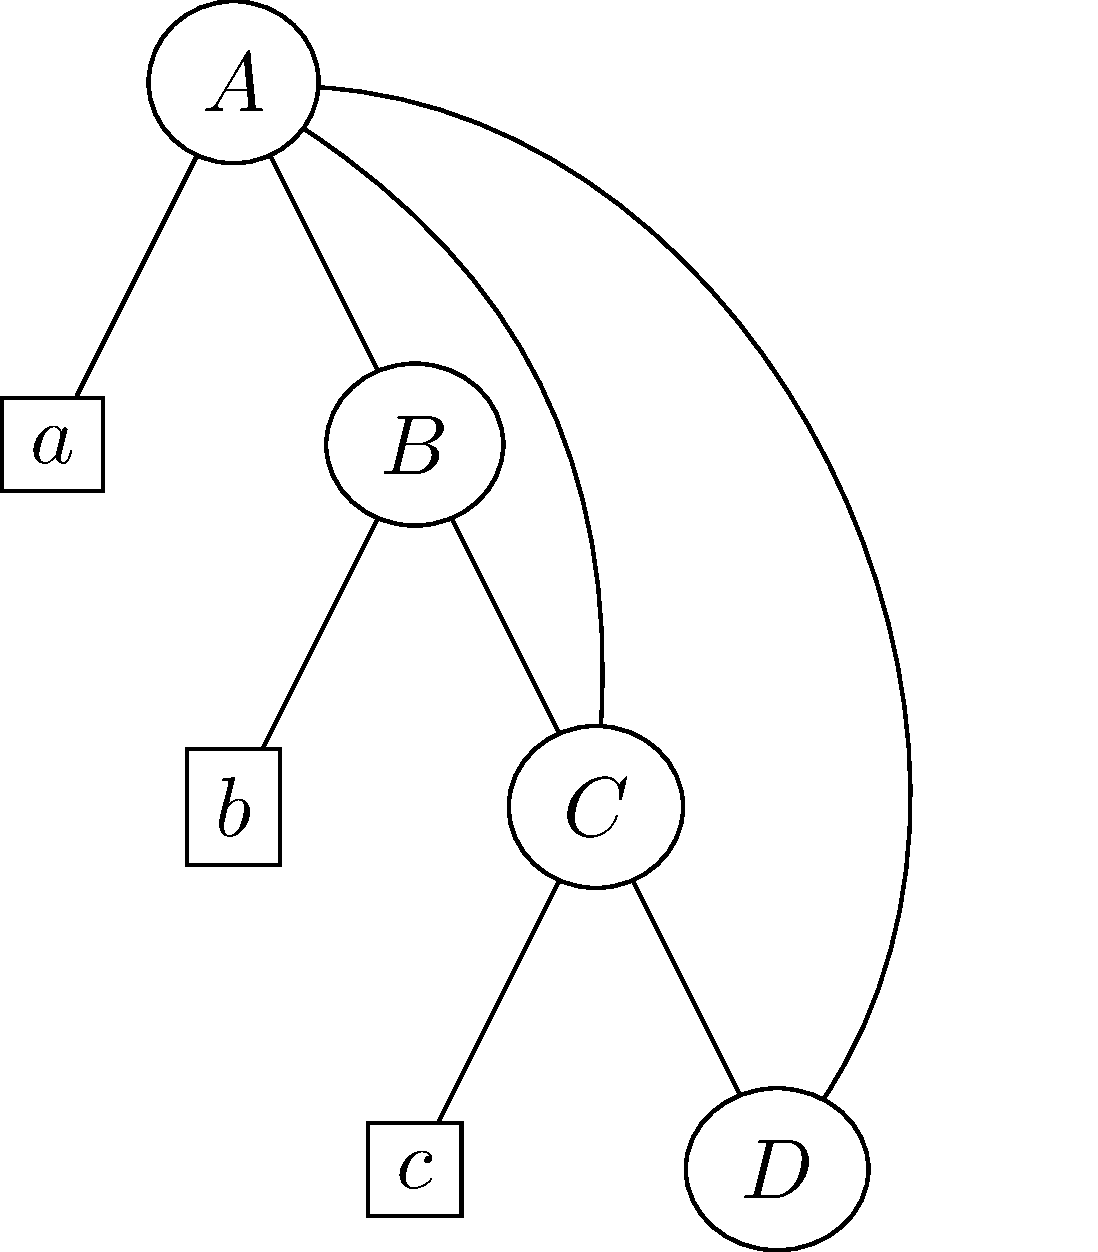
\includegraphics[height=.6\textheight]{../imgs/example_antisthenis_dag.pdf}
      \end{center}
    \end{column}
  \end{columns}
\end{frame}
